\documentclass[12pt,aspectratio=169]{beamer}
\usetheme{metropolis}
\setbeamersize{text margin left=.5cm,text margin right=.5cm}
\usepackage[lf]{carlito}
\usepackage{siunitx}
\usepackage{tikz}
\usepackage{mathpazo}
\usepackage{bm}
\usepackage{mathtools}
\usepackage[ISO]{diffcoeff}
\diffdef{}{ op-symbol=\mathsf{d} }
\usepackage{xcolor,colortbl}

\setmonofont{Ubuntu Mono}
\setlength{\parskip}{0pt}
\renewcommand{\baselinestretch}{1}

\sisetup{
  inter-unit-product=\cdot,
  per-mode=symbol
}

\tikzset{
  >=latex
}

%\newcommand{\iii}{\hat{\bm\imath}}
%\newcommand{\jjj}{\hat{\bm\jmath}}
%\newcommand{\kkk}{\hat{\bm k}}


\setlength{\parskip}{0pt}
\renewcommand{\baselinestretch}{1}

\sisetup{
  inter-unit-product=\cdot,
  per-mode=symbol
}
\tikzset{>=latex}

\title{Topic 11: Electrostatics}
\subtitle{Advanced Placement Physics C}
\author[TML]{Dr.\ Timothy Leung}
\institute{Olympiads School}
\date{Updated: Summer 2022}

\newcommand{\pic}[2]{
  \includegraphics[width=#1\textwidth]{#2}
}
\newcommand{\eq}[2]{
  \vspace{#1}{\Large
    \begin{displaymath}
      #2
    \end{displaymath}
  }
}
%\newcommand{\iii}{\ensuremath\hat{\bm{\imath}}}
%\newcommand{\jjj}{\ensuremath\hat{\bm{\jmath}}}
%\newcommand{\kkk}{\ensuremath\hat{\bm{k}}}
\newcommand{\iii}{\ensuremath\hat\imath}
\newcommand{\jjj}{\ensuremath\hat\jmath}
\newcommand{\kkk}{\ensuremath\hat k}



\begin{document}

\begin{frame}
  \maketitle
\end{frame}


\section{Electrostatic Force}

\begin{frame}{Review: The Charges Are}
  We should already know a bit about charge particles:
  \begin{itemize}
  \item A \textbf{proton} carries a \textbf{positive} charge
  \item An \textbf{electron} carries a \textbf{negative} charge
  \item A \emph{net charge} of an object means an excess of protons or electrons
  \item Similar charges are repel; opposite charges attract
  \end{itemize}

  \vspace{.2in}We start with electrostatics:
  \begin{itemize}
  \item Charges that are not moving relative to one another
  \end{itemize}
\end{frame}



\begin{frame}{Coulomb's Law for Electrostatic Force}
  \begin{center}
    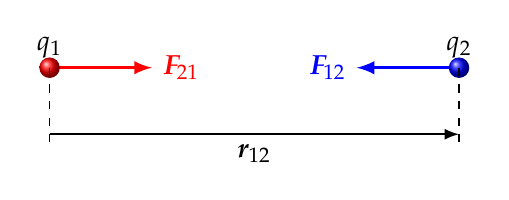
\begin{tikzpicture}[scale=.65]
      \begin{scope}[->,very thick]
        \draw[red] (0,0)--(2,0) node[right]{$\bm{F}_{21}$};
        \draw[blue](8,0)--(6,0) node[left] {$\bm{F}_{12}$};
      \end{scope}
      \tikzstyle{balloon1}=[ball color=red];
      \tikzstyle{balloon2}=[ball color=blue];
      \shade[balloon1] (0,0) circle(.2) node[above]{$q_1$};
      \shade[balloon2] (8,0) circle(.2) node[above]{$q_2$};
      \draw[dashed] (0,0)--(0,-1.5);
      \draw[dashed] (8,0)--(8,-1.5);
      \draw[->,thick](0,-1.3)--(8,-1.3) node[midway,below]{$\bm{r}_{12}$};
    \end{tikzpicture}
  \end{center}
  The \textbf{electrostatic force} (or \textbf{coulomb force}) is a mutually
  repulsive/attractive force between all charged objects. The force that charge
  $q_1$ exerts on $q_2$ is given by \textbf{Coulomb's law}:

  \eq{-.2in}{
    \boxed{\bm{F}_{12}=\frac{kq_1q_2}{|\bm{r}_{12}|^2}\hat{\bm{r}}_{12}}
  }
\end{frame}



\begin{frame}{Coulomb's Law for Electrostatic Force}
  \eq{-.2in}{
    \boxed{\bm{F}_{12}=\frac{kq_1q_2}{|\bm{r}_{12}|^2}\hat{\bm{r}}_{12}}
  }
  \begin{center}
    \begin{tabular}{l|c|c}
      \rowcolor{pink}
      \textbf{Quantity} & \textbf{Symbol} & \textbf{SI Unit} \\ \hline
      Electrostatic force            & $\bm{F}_{12}$ & \si{\newton} \\
      Coulomb's constant (electrostatic constant) & $k$ & \si{N.m^2/C^2} \\
      Point charges 1 and 2  & $q_1$, $q_2$ &  \si{\coulomb} \\
      Distance between point charges & $|\bm{r}_{12}|$ & \si{\metre} \\
      Unit vector of direction between point charges & $\hat{\bm{r}}_{12}$ &
    \end{tabular}
  \end{center}

  \vspace{-.1in}\textbf{Coulomb's constant}
  $\displaystyle k=\frac1{4\pi\epsilon_0}=\SI{8.99e9}{N.m^2/C^2}$ where
  $\epsilon_0=\SI{8.85e-12}{C^2/N.m^2}$ is called the
  ``permittivity of free space''
\end{frame}



\begin{frame}{Coulomb's Law for Electrostatic Force}
  \begin{center}
    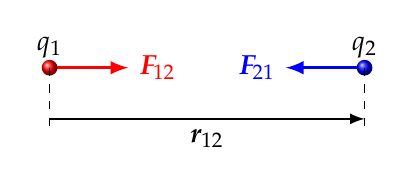
\begin{tikzpicture}[scale=.5]
      \begin{scope}[->,very thick]
        \draw[red] (0,0)--(2,0) node[right]{$\bm{F}_{12}$};
        \draw[blue](8,0)--(6,0) node[left] {$\bm{F}_{21}$};
      \end{scope}
      \tikzstyle{balloon1}=[ball color=red];
      \tikzstyle{balloon2}=[ball color=blue];
      \shade[balloon1] (0,0) circle(.2) node[above]{$q_1$};
      \shade[balloon2] (8,0) circle(.2) node[above]{$q_2$};
      \draw[dashed] (0,0)--(0,-1.5);
      \draw[dashed] (8,0)--(8,-1.5);
      \draw[->,thick](0,-1.3)--(8,-1.3) node[midway,below]{$\bm{r}_{12}$};
    \end{tikzpicture}
  \end{center}
  \begin{itemize}
  \item\vspace{-.15in}If $q_1$ exerts an electrostatic force $\bm{F}_{12}$ on
    $q_2$, then $q_2$ likewise exerts a force of $\bm{F}_{21}=-\bm{F}_{12}$
    on $q_1$. The two forces are equal in magnitude and opposite in direction
    (3rd law of motion).
  \item $q_1$ and $q_2$ are assumed to be \emph{point charges} that do not
    occupy  any space
  \item The (more familiar) scalar form is often used as well:

    \eq{-.2in}{
      \boxed{F_q=\frac{kq_1q_2}{r^2}}
    }
  \end{itemize}
\end{frame}



\begin{frame}{More Than One Charge}
  \begin{columns}
    \column{.4\textwidth}
    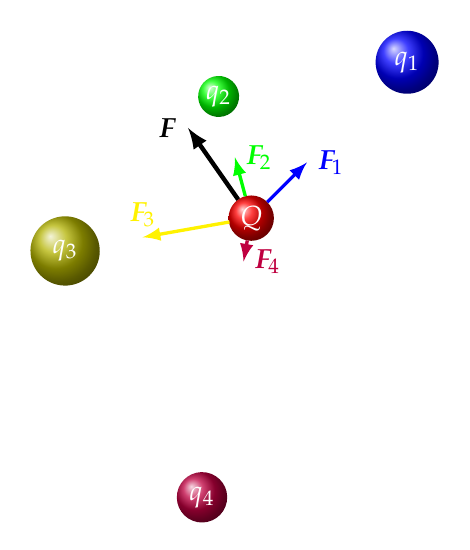
\begin{tikzpicture}[scale=.4]
      \tikzstyle{balloon1}=[ball color=red];
      \tikzstyle{balloon2}=[ball color=blue];
      \tikzstyle{balloon3}=[ball color=green];
      \tikzstyle{balloon4}=[ball color=yellow!70!black];
      \tikzstyle{balloon5}=[ball color=purple];
      \shade[balloon1] (0,0) circle(.72) node[white]{$Q$};
      \begin{scope}[rotate=45]
        \draw[->,very thick,blue](.72,0)--(2.5,0) node[right]{$\bm{F}_1$};
        \shade[balloon2] (7,0) circle(1) node[white]{$q_1$};
      \end{scope}
      \uncover<2->{
        \begin{scope}[rotate=105]
          \draw[->,very thick,green](.72,0)--(2,0)
          node[right]{$\bm{F}_2$};
          \shade[balloon3] (4,0) circle(.65) node[white]{$q_2$};
        \end{scope}
      }
      \uncover<3->{
        \begin{scope}[rotate=190]
          \draw[->,very thick,yellow](.7,0)--(3.5,0)
          node[above]{$\bm{F}_3$};
          \shade[balloon4] (6,0) circle(1.1) node[white]{$q_3$};
        \end{scope}
      }
      \uncover<4->{
        \begin{scope}[rotate=260]
          \draw[->,very thick,purple](.72,0)--(1.4,0)
          node[right]{$\bm{F}_4$};
          \shade[balloon5] (9,0) circle(.8) node[white]{$q_4$};
        \end{scope}
      }
      \uncover<5>{
        \begin{scope}[rotate=125]
          \draw[->,ultra thick](.72,0)--(3.5,0) node[left]{$\bm{F}$};
        \end{scope}
      }
    \end{tikzpicture}

    \column{.6\textwidth}
    For a charge $Q$ that is subjected to the influence of multiple discrete
    point charges $q_i$, the total electrostatic force that $Q$ experiences is
    the vector sum of all the forces $\bm{F}_i$:
    
    \eq{-.25in}{
      \boxed{\bm{F}
        =\sum_i\bm{F}_i
        =kQ\left(\sum_{i=1}^N\frac{q_i}{r_i^2}\hat{\bm{r}_i}\right)
      }
    }
  \end{columns}
\end{frame}



\begin{frame}{Continuous Distribution of Charges}
  As $N\rightarrow\infty$, the summation becomes an integral, and can now be
  used to describe the force from charges with \emph{spatial extend} i.e.\
  charges that take up physical space (e.g.\ a continuous distribution of
  charges):

  \eq{-.2in}{
    \boxed{\bm{F}
      =\int\dl\bm{F}
      =kQ\int\frac{\dl q}{r^2}\hat{\bm{r}}
    }
  }
\end{frame}



\section{Electric Field}

\begin{frame}{Electric Field}
  The expression for \textbf{electric field} is obtained by repeating the same
  procedure as with gravitational field, by grouping the variables in
  Coulomb's law:

  \eq{-.2in}{
    F_q
    =\underbrace{
      \left[\frac{kq_1}{|\bm{r}_{12}|^2}\hat{\bm{r}}\right]
    }_{\bm{E}}q_2
  }

  \vspace{-.15in}The electric field $\bm{E}$ created by $q_1$ is a vector
  function (called a \textbf{vector field}) that shows how it influences other
  charged particles around it.
\end{frame}



\begin{frame}{Electric Field Near a Point Charge}
  The electric field a distance $r$ away from a point charge $q$ is given by:

  \eq{-.2in}{
    \boxed{\bm{E}(q,\bm{r})=\frac{kq}{|\bm{r}|^2}\hat{\bm{r}}}
  }
  \begin{center}
    \begin{tabular}{l|c|c}
      \rowcolor{pink}
      \textbf{Quantity} & \textbf{Symbol} & \textbf{SI Unit} \\ \hline
      Electric field intensity    & $\bm{E}$ & \si{\newton\per\coulomb}\\
      Coulomb's constant          & $k$   & \si{N.m^2/C^2} \\
      Source charge               & $q$   & \si{\coulomb} \\
      Distance from source charge & $|\bm{r}|$   & \si{\metre} \\
      Outward unit vector from point source & $\hat{\bm{r}}$ &
    \end{tabular}
  \end{center}
  The direction of $\bm{E}$ is radially outward from a positive point charge
  and radially inward towards a negative charge.
\end{frame}



\begin{frame}{More Than One Charge}
  When multiple point charges are present, the total electric field at any
  position $\bm{r}$ is the vector sum of all the fields $\bm{E}_i$:
    
  \eq{-.2in}{
    \boxed{\bm{E}
      =\sum_i\bm{E}_i
      =k\left(\sum_i\frac{q_i}{r_i^2}\hat{\bm{r}_i}\right)
    }
  }
\end{frame}



\begin{frame}{More Than One Charge}
  As $N\rightarrow\infty$, the summation becomes an integral, and can now be
  used to describe the electric field generated by charges with
  \emph{spatial extend}:

  \eq{-.2in}{
    \boxed{
      \bm{E}=\int\dl\bm{E}=k\int\frac{\dl q}{r^2}\hat{\bm{r}}
    }
  }
  
  This integral may be difficult to compute if the geometry of is complicated,
  but in general, there are usually symmetry that can be exploited.
\end{frame}



\begin{frame}{Think Electric Field}
  $\bm{E}$ itself \emph{doesn't do anything} until another charge interacts with
  it. And when there is a charge $q$, the electrostatic force $\bm{F}_q$ that
  the charge experiences is proportional to $q$ and $\bm{E}$, regardless of how
  the electric field is generated:

  \eq{-.3in}{
    \boxed{\bm{F}_q=q\bm{E}}
  }

  \vspace{-.15in}A positive charge in the electric field experiences a
  electrostatic force $\bm{F}$ in the same direction as $\bm{E}$.
\end{frame}



\begin{frame}{Electric Field Lines}
  %If you place a positive charge in an electric field, the electrostatic force
  %on the charge will be in the direction of the electric field.
  \begin{columns}
    \column{0.25\textwidth}
    \pic{.95}{pos_charge}\\
    \pic{.95}{neg_charge}
    \column{0.75\textwidth}
    \pic{.95}{2charges}
  \end{columns}
\end{frame}



\begin{frame}{Lord of the Ring Charge}
  Suppose you have been given \emph{The One Ring To Rule Them All}, and you
  found out that it is charged! What is its electric field at point $P$ along
  its axis?
  \begin{center}
    \pic{.5}{physicsbook_emism_graphik_35}
  \end{center}
  Note that calculating the electric field away from the axis is very
  difficult.
\end{frame}



\begin{frame}{Electric Field Along Axis of a Ring Charge}
  \begin{columns}
    \column{.3\textwidth}
    \vspace{.1in}
    \pic{1.1}{Fig25}

    \column{.7\textwidth}
    \begin{itemize}
    \item We can separate the electric field $\dl\bm{E}$ (generated by charge
      $\dl q$) into axial ($\dl E_x$) and radial ($\dl E_\perp$) components
    \item Based on symmetry, $\dl E_\perp$ doesn't contribute to anything; but
      $\dl E_x$ is pretty easy to find:

    \end{itemize}
  \end{columns}
  \eq{-.1in}{
    \dl E_x =\frac{k\dl q}{r^2}\cos\theta=\frac{k\dl q}{r^2}\frac xr
    =\frac{kx\dl q}{(x^2+a^2)^{3/2}}
  }      

  \vspace{-.15in}Integrating this over all charges $\dl q$, we have:
  
  \eq{-.25in}{
    E_x =\frac{kx}{(x^2+a^2)^{3/2}}\int \dl q=\boxed{\frac{kQx}{(x^2+a^2)^{3/2}}}
  }
\end{frame}




\begin{frame}{Electric Field Along Axis of a Uniformly Charged Disk}
  Let's extend what we know to a disk of radius $a$ and charge density $\sigma$

  \vspace{.1in}
  \begin{columns}
    \column{.37\textwidth}
    \pic{1}{serway}

    \column{.63\textwidth}
    We start with the solution from the ring problem, and replace $Q$ with
    $\dl q=2\pi\sigma a\dl a$:

    \eq{-.2in}{
      \dl E_x =\frac{2\pi kx\sigma a}{(x^2+a^2)^{3/2}}\dl a
    }

    Integrating over the entire disk:

    \eq{-.2in}{
      E_x =\pi kx\sigma\int\frac{2a}{(x^2+a^2)^{3/2}}\dl a
    }
    
    This is not an easy integral!
  \end{columns}
\end{frame}



\begin{frame}{Eclectic Field Along Axis of a Uniformly Charged Disk}
  \begin{columns}
    \column{.3\textwidth}
    \pic{1.2}{serway}
    
    \column{.67\textwidth}
    \begin{itemize}
    \item Luckily for us, the integral is in the form of $\int u^ndu$, with
      $u=x^2+a^2$ and $n=\frac{-3}2$.
    \item You can find the integral in any math textbook:

      \eq{-.3in}{
        \boxed{E_x =2\pi k\sigma\left(1-\frac{x}{\sqrt{x^2+R^2}}\right)}
      }
      \end{itemize}
  \end{columns}
\end{frame}



\section{Gauss's Law}

\begin{frame}{Flux}
  \textbf{Flux} is an important concept in many disciplines in physics. The
  flux of a vector quantity $\bm{X}$ is the amount of that quantity flowing
  through a surface. In integral form:

  \eq{-.2in}{
    \Phi=\int\bm{X}\cdot\dl\bm{A}\quad\text{or}\quad
    \Phi=\int(\bm{X}\cdot\bm{\hat{n}})\dl A
  }

  The direction of the infinitesimal area $\dl\bm{A}$ is \textbf{outward normal}
  to the surface.
  \begin{center}
    \pic{.3}{eflux}
  \end{center}
\end{frame}



\begin{frame}{Flux}
  \vspace{.2in}$\Phi$ can be something physical, like water, or bananas, or
  something abstract, like electric field (which is what we are interested
  in). We can compute a flux as long as there is a vector field i.e.\
  $\bm{X}=\bm{X}(x,y,z)$. In the case of \textbf{electric flux}, the quantity
  $\bm{X}$ is just the
  electric field, i.e.:
    
  \eq{-.2in}{
    \Phi_q=\int\bm{E}\cdot\dl\bm{A}
  }
  \begin{center}
    \pic{.3}{eflux}
  \end{center}
\end{frame}



\begin{frame}{Electric Flux and Gauss's Law}
  \textbf{Gauss's law} tells us that if we have a closed surface (think of
  the surface of a balloon), the total electric flux is very well defined:

  \eq{-.2in}{
    \boxed{
      \Phi_q=\oint\bm{E}\cdot\dl\bm{A}=\frac{Q_\text{encl}}{\epsilon_0}
    }
  }
    
  where
  \begin{itemize}
  \item $Q_\text{encl}$ is the charge enclosed by the surface
  \item $\epsilon_0=\SI{8.85e-12}{C^2/N.m^2}$ is the permittivity of free space
  \end{itemize}
  That closed surface is called a \textbf{Gaussian surface}
\end{frame}



\begin{frame}{Closed Surfaces}
  \begin{columns}
    \column{.55\textwidth}
    A \textbf{closed surface} is one that does not have a boundary, like the
    sphere, toroid, and cube on the left.
    \column{.45\textwidth}
    \pic{1}{800px-SurfacesWithAndWithoutBoundary}
  \end{columns}
\end{frame}



\begin{frame}{Electric Field from a Positive Point Charge}
  \begin{columns}
    \column{.25\textwidth}
    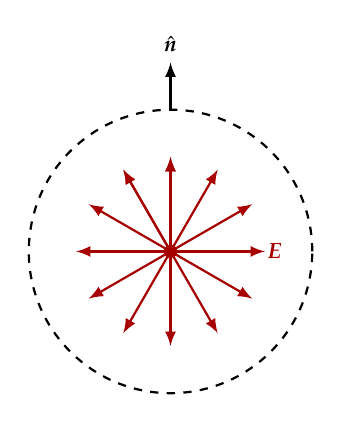
\begin{tikzpicture}[scale=1.2]
      \fill[red!65!black](0,0) circle(0.07);
      \draw[dashed,thick](0,0) circle(1.5);
      \foreach \x in {0,...,13}{
        \draw[red!65!black,thick,rotate=30*\x,->](0,0)--(0,1);
      }
      \draw[thick,->](0,1.5)--(0,2)
      node[above]{\footnotesize$\hat{\bm{n}}$};
      \node[red!65!black] at (1.1,0) (E) {\footnotesize$\bm{E}$};
    \end{tikzpicture}
    
    \column{.75\textwidth}
    By symmetry, electric field lines must be radially outward from the charge,
    so the integral reduces to:

    \eq{-.2in}{
      \Phi_q=\oint\bm{E}\cdot\dl\bm{A}=EA=\frac{q}{\epsilon_0}
    }

    Since area of a sphere is $A=4\pi r^2$, we recover Coulomb's law and the
    magnitude of the electric field from a point charge:

    \eq{-.2in}{
      E=\frac{1}{4\pi\epsilon_0}\frac{q}{r^2}=\frac{kq}{r^2}
    }
  \end{columns}
\end{frame}




\section{Electric Potential \& Potential Energy}

\begin{frame}{Electrical Potential Energy}
  The work done by the electrostatic force is given by:
  
  \eq{-.3in}{
    W=\int\bm{F}_q\cdot\dl\bm{r}
    =kq_1q_2\int_{r_1}^{r_2}\frac1{r^2}\dl r
    =-\frac{kq_1q_2}{r}\Big|^{r_2}_{r_1}=-\Delta U_q
  }

  where $Q_q$ is defined as the \textbf{electric potential energy}:
    
  \eq{-.2in}{
    \boxed{U_q=\frac{kq_1q_2}{r}}
  }

  $U_q$ can be ($+$) or ($-$), because charges can be either ($+$) or ($-$).
\end{frame}



\begin{frame}{How it Differs from Gravitational Potential Energy}
  \begin{columns}
    \column{.33\textwidth}
    \centering
    Two positive charges:

    \eq{-.3in}{U_q>0}
    
    \column{.33\textwidth}
    \centering
    Two negative charges:

    \eq{-.3in}{U_q>0}
    
    \column{.34\textwidth}
    \centering
    One positive and one negative charge:

    \eq{-.5in}{U_q<0}
  \end{columns}
  \begin{itemize}
  \item $U_q>0$ means positive work is done to bring two charges together from
   $r=\infty$ to $r$ (both charges of the same sign)
  \item $U_q<0$ means negative work (the charges are opposite signs)
  \item For gravitational potential $U_g$ is always $<0$
  \end{itemize}
\end{frame}



\begin{frame}{Electric Potential}
  When I move an object of mass $m$ against a gravitational force from one
  point to another, the work that I do is directly proportional to $m$, i.e.\
  there is a ``constant'' in that scales with \emph{any} mass, as long as they
  move between those same two points:

  \eq{-.2in}{
    U_g=Km
  }

  In the trivial case (small changes in height, no change in $g$), this
  constant is just

  \eq{-.2in}{
    \frac{U_g}m=g\Delta h
  }
\end{frame}



\begin{frame}{Electric Potential}
  This is also true for moving a charged particle $q$ against an electric
  electric field created by $q_s$, and the ``constant'' is called the
  \textbf{electric potential}. For a point charge, it is defined as:

  \eq{-.2in}{
    \boxed{V=\frac{U_q}q=\frac{kq_s}r}
  }

  The unit for electric potential is a \emph{volt} which is
  \emph{one joule per coulomb}:

  \eq{-.2in}{
    \SI1\volt=\SI1{\joule\per\coulomb}
  }

  \vspace{-.2in}We can easily the relationship between $V$ and $\bm{E}$:
  
  \eq{-.2in}{
    \boxed{\Delta V=\int\bm{E}\cdot\dl\bm{r}}
  }
\end{frame}



\begin{frame}{Potential Difference (Voltage)}

  The change in electric potential is called the
  \textbf{electric potential difference} or \textbf{voltage}:

  \eq{-.2in}{
    \boxed{\Delta V=\frac{\Delta U_q}{q}}\quad\textsf{\normalsize and}\quad
    \boxed{\dl V=\frac{\dl U_q}{q}}
  }

  Here, we can relate $\Delta V$ to an equation that we knew from Grade 11
  Physics, which related to the energy dissipated in a resistor in a circuit
  $\Delta U$ to the voltage drop $\Delta V$:
    
  \eq{-.2in}{
    \boxed{\Delta U_q=q\Delta V}
  }

  Electric potential difference also has the unit \emph{volts} (\si{\volt})
\end{frame}



\begin{frame}{Getting Those Names Right}
  Remember that these three scalar quantities, as opposed to electrostatic
  force $\bm{F}_q$ and electric field $\bm{E}$ which are vectors
  \begin{itemize}
  \item Electric potential energy:
    \begin{displaymath}
      U=\frac{kq_1q_2}{r}
    \end{displaymath}
  \item Electric potential:
    \begin{displaymath}
      V=\frac{kq}{r}
    \end{displaymath}
  \item Electric potential difference (voltage):
    \begin{displaymath}
      \Delta V=\frac{\Delta U_q}{q}
    \end{displaymath}
  \end{itemize}
\end{frame}


\begin{frame}{Relating $U_q$, $\bm{F}_q$ and $\bm{E}$}{Our Integrals In Reverse}
  From the fundamental theorem calculus, we can relate electrostatic force
  ($\bm{F}_q$) to electric potential energy ($U_q$) by the gradient operator,
  and electric field ($\bm{E}$) to the electric potential ($V$) the same way:

  \eq{-.2in}{
    \bm{F}_q=-\nabla U_q=-\diffp{U_q}r\hat{\bm{r}}
    \quad\;\;
    \bm{E}=-\nabla V=-\diffp Vr\hat{\bm{r}}
  }
  \begin{itemize}  
  \item Electrostatic force $\bm{F}_q$ always points from high to
    low potential energy (steepest descent direction)
  \item Electric field can also be expressed as the change of electric
    potential per unit distance, which has the unit
    
    \eq{-.2in}{
      \SI{1}{\newton\per\coulomb}=\SI{1}{\volt\per\metre}
    }
  \item Electric field is also called ``potential gradient''
  \end{itemize}
\end{frame}



\begin{frame}{Equipotential Lines}
  \begin{center}
    \pic{0.65}{plate3}
  \end{center}
  The dotted blue lines are called \textbf{equipotential lines}. They are
  always \emph{perpendicular} to the electric field lines. Charges moving in
  the direction of the equipotential lines have constant electric potential
\end{frame}



\begin{frame}{Electric Field Near an Infinite Plane of Charge}
  \begin{columns}
    \column{.25\textwidth}
    \pic{1.1}{elec_gauss_figure9}

    \column{.75\textwidth}
    \begin{itemize}
    \item Charge density (charge per unit area) $\sigma$
    \item By symmetry, $\bm{E}$ must be perpendicular to the plane
    \item Our Gaussian surface is a cylinder shown in the left with an area
      $A$; the height of the cylinder is unimportant
    \item Nothing ``flows out'' of the side of the cylinder, only at the ends
    \item The total flux is $\Phi_q=E(2A)$
    \item The enclosed charge is $Q_\text{encl}=\sigma A$
    \end{itemize}
  \end{columns}
\end{frame}



\begin{frame}{Electric Field Near an Infinite Plane of Charge}
  \begin{columns}
    \column{.25\textwidth}
    \pic{1.1}{elec_gauss_figure9}

    \column{.75\textwidth}
    Gauss's law simplifies to:
    
    \eq{-.2in}{
      \oint\bm{E}\cdot\dl\bm{A}=\frac{Q_\text{encl}}{\epsilon_0}
      \;\rightarrow\;
      E(2A)=\frac{\sigma A}{\epsilon_0}
    }

    \vspace{-.1in}Solving for $E$, we get:

    \eq{-.2in}{
      \boxed{E=\frac{\sigma}{2\epsilon_0}}
    }
    \begin{itemize}
    \item $E$ is a constant
    \item Independent of distance from the plane
    \item Both sides of the plane are the same
    \end{itemize}
  \end{columns}
\end{frame}



\begin{frame}{Electric Field Between Parallel Charged Plates}
  \begin{center}
    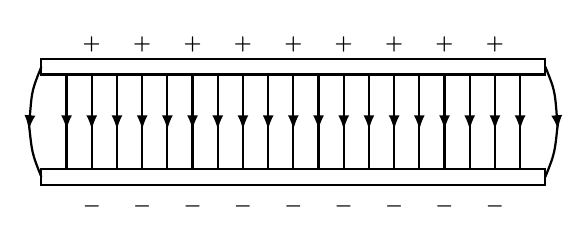
\begin{tikzpicture}[xscale=.8]
      \begin{scope}[thick]
        \draw(0,0) rectangle (8,.2);
        \draw(0,1.4) rectangle (8,1.6);
        \foreach \x in {.4,.8,1.2,...,7.6}{
          \draw[->](\x,1.4)--(\x,.7);
          \draw    (\x,1.4)--(\x,.2);
        }
        \foreach \x in {.8,1.6,2.4,...,7.2}{
          \node at (\x,1.78) {\scriptsize $\bm{+}$};
          \node at (\x,-.28) {\scriptsize $\bm{-}$};
        }
        
        \draw[->] (0,1.5)..controls(-.15,1.2)..(-.2,.7);
        \draw (-.2,.8)..controls(-.15,.4)..(0,.1);
        
        \draw[->](8,1.5)..controls(8.15,1.2)..(8.2,.7);
        \draw    (8.2,.8)..controls(8.15,.4)..(8,.1);
      \end{scope}
    \end{tikzpicture}
  \end{center}
  \begin{itemize}
  \item Two plates, each producing an electric field pointing in
    the same direction
  \item The total electric field is twice the value of \emph{one} infinite
    plane, pointing from the positively charged plate towards the negatively
    charged plate

    \eq{-.2in}{
      \boxed{E=\frac{\sigma}{\epsilon_0}}
    }
  \item $\bm{E}$ outside the plates is very low (close to zero), except for
    fringe effects at the edges of the plates
  \end{itemize}
\end{frame}



\begin{frame}{Electric Field and Electric Potential Difference}
  Recall the relationship between electric field ($\bm{E}$) and electric
  potential difference ($V$):
    
  \eq{-.2in}{
    \bm{E}=-\diffp Vr\hat{\bm{r}}
  }
  
  This relationship holds regardless of the charge configuration.
\end{frame}




\begin{frame}{Electric Field and Electric Potential Difference}
  \begin{center}
    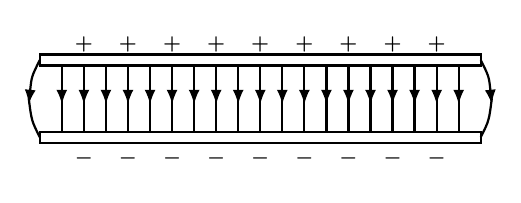
\begin{tikzpicture}[scale=.7]
      \begin{scope}[thick]
        \draw(0,0) rectangle (8,.2);
        \draw(0,1.4) rectangle (8,1.6);
        \foreach\x in {.4,.8,1.2,...,7.6}{
          \draw[->](\x,1.4)--(\x,.7);
          \draw(\x,1.4)--(\x,.2);
        }
        \foreach\x in {.8,1.6,2.4,...,7.2}{
          \node at (\x,1.78) {\scriptsize $\bm{+}$};
          \node at (\x,-.28) {\scriptsize $\bm{-}$};
        }
        
        \draw[->](0,1.5)..controls(-.15,1.2)..(-.2,.7);
        \draw(-.2,.8)..controls(-.15,.4)..(0,.1);
        
        \draw[->](8,1.5)..controls(8.15,1.2)..(8.2,.7);
        \draw(8.2,.8)..controls(8.15,.4)..(8,.1);
      \end{scope}
    \end{tikzpicture}
  \end{center}
  In the case of two parallel plates, the electric field is uniform, and the
  relationship simplifies to:

  \eq{-.2in}{
    \boxed{E=\frac{\Delta V}d}
  }
  \begin{center}
    \begin{tabular}{l|c|c}
      \rowcolor{pink}
      \textbf{Quantity} & \textbf{Symbol} & \textbf{SI Unit} \\ \hline
      Electric field intensity & $E$ & \si{\newton\per\coulomb}\\
      Electric potential difference between plates & $\Delta V$ &
      \si{\volt} \\
      Distance between plates       & $d$ & \si{\metre}
    \end{tabular}
  \end{center}
\end{frame}
\end{document}
